\enteteExam{NFP 107 -- Systèmes de gestion de bases de données - Durée 2h30}%
{Examen FOAD session 1 -- 21 janvier 2026}%
{Documents autorisés\,: 10 pages de notes manuscrites ou imprimées}%

Essayons de modéliser un système  qui permet d'emprunter 
un réseau de transport en comptabilisant les passages. Le réseau
est organisé en \emph{lignes} desservant plusieurs \emph{stations}, chaque station peut être commune
à plusieurs lignes (ce qui permet des changements). Les abonnés ont une carte
qu'ils valident à l'entrée dans une station et à la sortie dans une autre, ce qui
constitue un \emph{trajet}. 


Un concepteur propose le schéma suivant; les clés primaires sont en gras.

\begin{itemize}
\item Abonné(\textbf{id}, nom, prénom, noMobile)
\item Ligne (\textbf{id}, intitulé)
\item Station(\textbf{id}, nom)
\item DétailLigne(\textbf{id}, idLigne, idStation, idStationSuivante)
\item Trajet(\textbf{id}, jour, idAbonné, idStationDépart, idStationArrivée)
\end{itemize}


Les jours sont répresentés simplement sous la forme 'jj/mm/aaaa', par exemple '14/01/2023'.

\subsection*{Conception du schéma (8 pts)}

\begin{enumerate}
   \item Quelles sont les clés étrangères\,?

 \item Aurait-on pu choisir comme clé de la table \texttt{Trajet}
      la paire d'attributs \texttt{(idAbonné, idStationDépart)}\,? Donnez vos arguments pour ou contre
      un tel changement.
       
  \item Le schéma permet-il de savoir par quelles lignes est passé un abonné pendant un trajet\,?
  
 \item Donnez les commandes SQL de création des tables \texttt{Ligne}, \texttt{Station}
 et \texttt{DétailLigne}. Notez que dans l'esprit du concepteur, 
 tous les attributs de \texttt{DétailLigne} 
 sont  \texttt{not null}.
  
  \item Indiquez comment exprimer la contrainte suivante\,:
         deux abonnés différents ne peuvent pas avoir le même
             numéro de mobile.
            
  \item Qu'est ce qui caractérise la tête d'une ligne (sa première station) et son terminus\,? 
      Aide\,: réflechissez aux valeurs (ou absences de valeur) possibles de l'attribut \texttt{idStationSuivante}
      dans la table \texttt{DétailLigne}.
 
  \item Quel est d'après vous le schéma entité-association 
        correspondant à ce schéma relationnel\,?
        
   \item On ajoute des informations relatives aux conducteurs, chaque conducteur étant 
      affecté chaque jour à une ligne. On identifie les dépendances fonctionnelles suivantes\,:
      \begin{itemize}
        \item $matriculeConducteur \to nom, pr\acute{e}nom$
        \item $matriculeConducteur, jour \to idLigne$
      \end{itemize}
      Quelles sont les modifications apportées au schéma relationnel\,?

\end{enumerate}

   
\begin{solution}
\begin{enumerate}
 \item L'attribut \texttt{idAbonné}, \texttt{idLigne} et  les trois attributs \texttt{idStation***}
 \item Non, cela reviendrait à imposer qu'un abonné parte d'une station une seule fois, et ce n'est 
      vraiment pas raisonnable...
    \item Non, on connaît les stations de départ et d'arrivée pour un trajet, mais la station
       ne détermine pas la ligne.
  
 \item Pour \texttt{DétailLigne}.
\begin{minted}{sql}
create table DétailLigne (id integer not null,
                          idLigne integer not null,
                          idStation integer not null, 
                          idStationSuivante integer not null,
                          primarykey (id),
                          foreign key (idLigne) references Ligne(id),
                          foreign key (idStation) references Station(id),
                           foreign key (idStationSuivante) references Station(id)
              )
\end{minted}     
\item Le numéro de mobile est une clé candidate\,: on ajoute la contrainte \texttt{unique(noMobile)}
 
\item La tête d'une station est caractérisée par le fait que l'id de la station n'est pas une 
   des \texttt{idStationSuivante} pour la même ligne\,; le terminus est une station dans \texttt{DétailLigne}
   est la valeur de \texttt{idStationSuivante}  qui n'est
   pas \texttt{idStation} pour la même ligne.

 \item La figure~\ref{reseau} montre le schéma E/A.
   \begin{figure}[htb]  
   \centerline{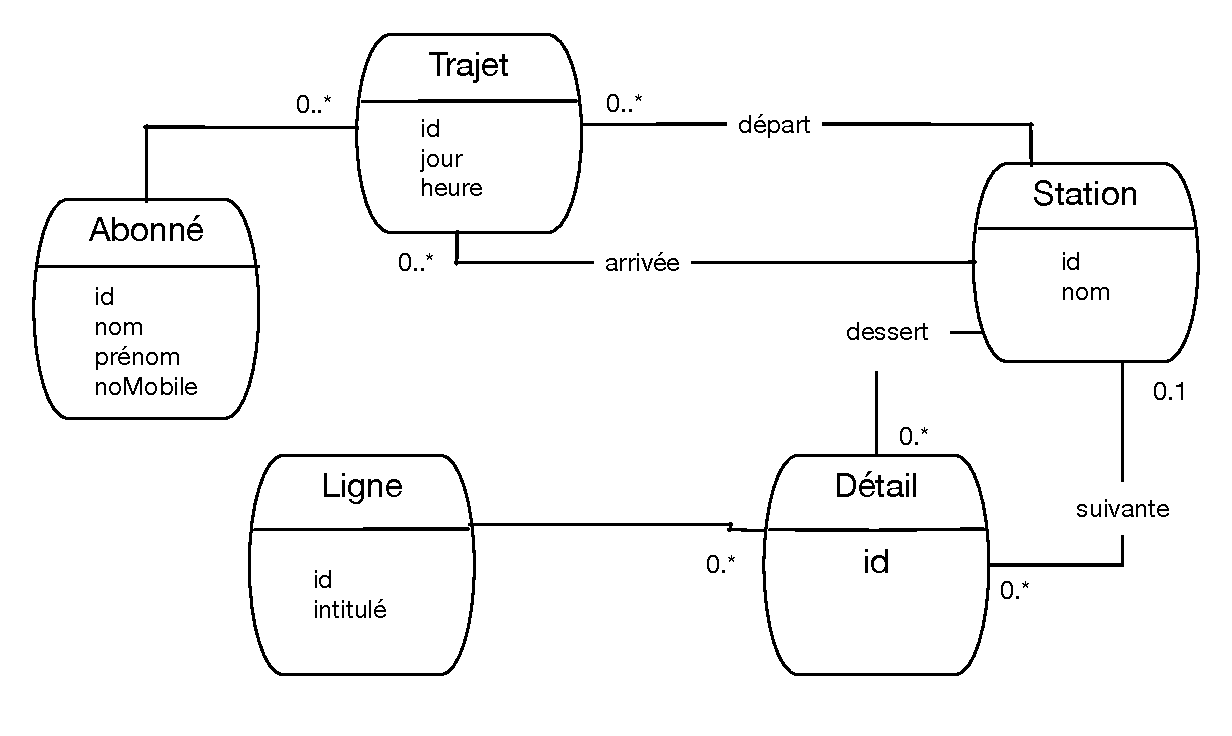
\includegraphics[scale=0.5]{../supports/figures/exam-23-reseau}}
    \caption{Modèle du réseau de transports}  
    \label{reseau}  
  \end{figure}  

\item On ajoute une table \texttt{Conducteur} et une table \texttt{Affectation(matricule,jour,idLigne)}
 dont la clé est la paire \texttt{(matricule,jour)}

  \end{enumerate}
\end{solution}


\subsection*{SQL (6 pts)}

Sur le schéma donné dans l'énoncé, exprimez en SQL les requêtes suivantes\,:

\begin{enumerate}
  \item Donnez la liste des trajets de l'abonné Philippe Rigaux, en affichant le jour, le nom
     de la station de départ et le nom de la station d'arrivée
  
  \item Quelles sont les stations où il est possible de passer de la ligne 'Rouge' à la ligne 'Jaune'
      (ce sont des intitulés)\,?
  
  \item Quelles sont les stations de la ligne 'Rouge' qui ne permettent aucun changement?
 
   \item Quelle est la station de tête de la ligne 'Rouge'\,?

%   \item Quel est le terminus de la ligne 'Rouge'\,?
   
   \item Donnez, pour chaque ligne, l'intitulé et le nombre de stations.
   \item Donnez les noms des abonnés qui  ont effectué plus de 4 trajets le 14 janvier 2023.
\end{enumerate}


   
\begin{solution}
\begin{enumerate}

 \item 
\begin{minted}{sql}
select t.jour, s1.npom as nomDépart, s2.nom as nomArivée 
from Trajet as t, Station as s1, Station as s2, Abonné as a
where a.prénom='Philippe' and a.nom='Rigaux'
and a.id = t.idAbonné
and s1.id = t.idStationDépart
and s2.id = t.idStationArrivée
\end{minted}     

  \item Quels sont les stations où il est possible de passer de la ligne 'Jaune'  à la ligne 'Rouge'
     (ce sont des intitulés)\,?
\begin{minted}{sql}
select s.nom
from Station as s, Ligne as l1, Ligne as l2, DétailLigne as d1, DétailLigne as d2
where s.id = d1.idStation
and s.id= d2.idStation
and d1.idLigne=l1.id
and d2.idLigne=l2.id
and l1.intitulé='Jaune'
and l2.intitulé='Rouge'
\end{minted}    

  \item Quelles sont les stations de la ligne 'Rouge' qui ne permettent aucun changement?
\begin{minted}{sql}
select s.nom
from Station as s, Ligne as l1,  DétailLigne as d1
where not exists (
      select * 
      from DétailLigne as d2
      where d2.idStation = s.id
      and   d2.idLigne != l1.idLigne)
ans s.id = d1.idStation
and d1.idLigne=l1.id
and l1.intitulé='Rouge'
\end{minted} 
   \item Quelle est la station de tête de la ligne 'Rouge'\,?
\begin{minted}{sql}
select s.nom
from Station as s, Ligne as l1,  DétailLigne as d1
where s.id not in (
      select d2.idStationSuivante
      from DétailLigne as d2
      where d2.idLigne = l1.id)
and s.id = d1.idStation
and d1.idLigne=l1.id
and l1.intitulé='Rouge'
\end{minted} 
   \item Donnez, pour chaque ligne, l'intitulé et le nombre de stations
\begin{minted}{sql}
select l.intitulé, count(*) as nbStations
from Station as s, Ligne as l1,  DétailLigne as d1
where s.id = d1.idStation
and d1.idLigne=l1.id
group by l.id, l.intitulé
\end{minted} 
   \item Donnez les noms des abonnés qui  ont effectué au moins 4 trajets le 14 janvier 2023.

\begin{minted}{sql}
   select a.nom, count(*) as nbTrajets
   from Abonné as a, Trajet as t
   where a.id = t.idAbonné
   and jour='14/01/2023'
   group by a.id, a.nom
   having count(*) >= 4
\end{minted}
   
\end{enumerate}


\end{solution}
\subsection*{Algèbre (2 pts)}

Donnez les expressions algébriques pour les requêtes suivantes

\begin{enumerate}
  \item Les stations qui ne sont sur aucune ligne 
  \item Les abonnés qui n'ont pas voyagé le 14 janvier 2023
\end{enumerate}


\subsection*{Vues (4 pts)}

La table \texttt{DétailLigne} ne représente la séquence
des stations que dans un seul sens. 
Par exemple, \texttt{DétailLigne} contient la
séquence des stations entre Balard et Créteil,
mais pas celle des stations entre Créteil et Balard.
Or, il est bien entendu
possible de parcourir une ligne dans les deux sens.

\begin{enumerate}
  \item Créer une vue \texttt{BiDirection} montrant 
      la séquence des stations d'une ligne dans les 
	  deux sens possibles. 
  \item En déduire la requête qui donne les
     deux stations immédiatement connexes à la station République,
	 sur la ligne \texttt{'Ligne 8'} (c'est son intitulé). 
	
\end{enumerate}

\begin{solution}
\begin{enumerate}
 \item La vue est l'union des séquences de stations
     dans \texttt{DétailLigne} et des séquences inversées.
\begin{minted}{sql}
create view  BiDirection as 
  select * from DetailLigne
    union
  select id, idLigne, idStation as idStationSuivante, 
       idStationSuivante as idStation
  from DetailLigne
\end{minted}     

 \item On interroge directement la vue sans avoir à se soucier
 du sens de parcours.
 

 \begin{minted}{sql}
    select s2.nom
    from Ligne as l, BiDirection as b, 
            Station as s, Station as s2
    where b.idLigne = l.id
    and  s.id = b.idStation
    and  s2.id = b.idStationSuivante
    and   l.intitulé = 'Ligne 8'
    and s.nom = 'République'
 \end{minted}

  \end{enumerate}
\end{solution}


%\subsection*{Procédures (2 pts)}

%\begin{enumerate}
%  \item Rappeler quelles sont les trois phases d'utilisation d'un curseur.
%  \item Expliquer ce que signifie l'immuabilité d'un curseur.
%\end{enumerate}

\end{document}

